\subsection{Pianificazione del lavoro}

\begin{figure}[H]
	\begin{center}
		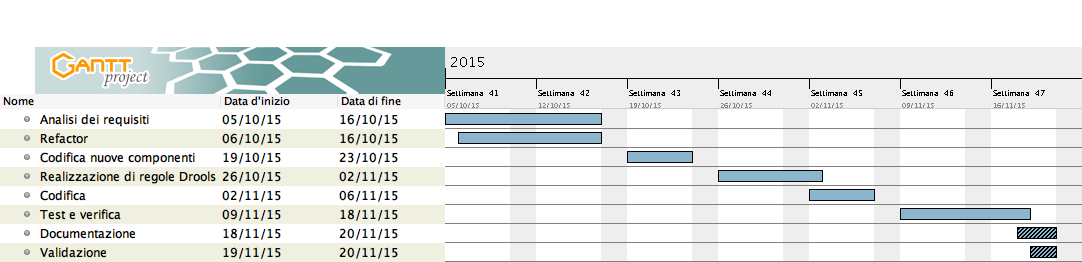
\includegraphics[width=16cm]{Pics/gantt.png}
		\caption{Diagramma di Gantt.}
		\label{fig:Gantt}
	\end{center}
\end{figure}


\hl{TODO Scrivo le cose relative al Gantt}

Durante lo stage, le ore sono state mantenute tali alle previsioni, la loro distribuzione nel tempo però è cambiata. Nello specifico l'ordine di esecuzione con le relative ore impiegate sono state le seguenti:
\begin{enumerate}
	\item	40 ore:     studio di Ruby on Rails, Drools e del software esistente;
	\item	20 ore:     rilevamento delle  criticità sulle componenti esistenti ;
	\item	30 ore:		analisi dei requisiti
	\item	15 ore:		riprogettazione delle componenti esistenti che presentano criticità
	\item	20 ore:     progettazione delle nuove entità richieste;
	\item	80 ore:     codifica di funzionalità e test;
	\item	4 ore:       colloquio con il committente per validare le nuove modifiche;
	\item 	4 ore:		 riprogettazione delle componenti da modificare;
	\item  	22 ore:	 	codifica di funzionalità e test;
	\item	40 ore:		implementazione delle regole Drools;
	\item 	15 ore:		 stesura della documentazione;
	\item	15 ore: 	verifica.
\end{enumerate}

Il numero totale delle ore di stage è 305.

 cose da dire:
 analisi e codifica spezzata in piu parti rispetto al previsto
Come è possibile osservare dalla lista, l'attività di progettazione è stata divisa in due parti distinte:  la prima relativa alle  componenti già presenti al momento dell'inizio dello stage, la seconda relativa alle nuove componenti.
 aumento del tempo dedicato ad analisi e codifica dovuto a modifiche committente
		=> sacrificati requisiti opzionali
 i test sono stati scritti durante la codifica
 



Alla fine della prima settimana è iniziata l'attività di analisi dei requisiti